\documentclass[11pt]{article}
\usepackage[margin=0.8in]{geometry}
\usepackage{graphicx,amsmath,booktabs,hyperref}
\title{HTT Observational Continuation: Conditional Results and Open Physical Laws}
\author{HTT observational analysis}
\date{14 October 2026}
\begin{document}\maketitle
\begin{abstract}This report uses one released DESI scalar BAO summary and one SMICA simulation diagnostic. It is not a three-probe joint fit, posterior, or native Bianchi-family result.\end{abstract}
\section{DESI scalar physical response}
The retained BGS Bright syst datum is $q_{\rm iso}=0.982880\pm0.018695$ at $z_{\rm eff}=0.295235$. In flat matter--$\Lambda$ FLRW with a free positive $H_0r_d$, $q_{\rm pred}=\frac{c}{H_0r_d}\frac{[zI(z)^2/E(z)]^{1/3}}{(D_V/r_d)_{\rm fid}}$, $I(z)=\int_0^z dz'/E(z')$ and $E(z)^2=\Omega_m(1+z)^3+1-\Omega_m$. At fixed $\Omega_m=0.30$, $H_0r_d=10,125.3\,\mathrm{km\,s^{-1}}$ maximizes the conditional Gaussian density, with pointwise 95\% inversion $[9,761.4,10,517.4]\,\mathrm{km\,s^{-1}}$. Every displayed $\Omega_m$ attains the same maximum by changing $H_0r_d$; this is no two-parameter posterior or raw-catalogue coverage result.
\begin{figure}[ht]\centering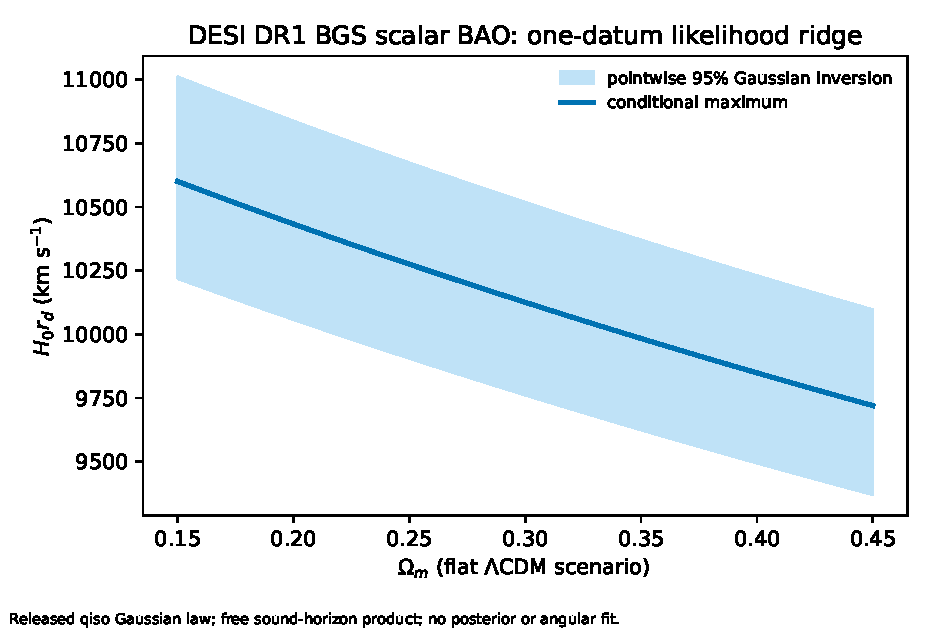
\includegraphics[width=.82\linewidth]{docs/observational_analysis_20261014/results/oa07_flatlcdm/flatlcdm_profile.pdf}\caption{One-datum conditional likelihood ridge. The band is a pointwise released-Gaussian inversion, not a posterior.}\end{figure}
\section{CMB same-operator simulation diagnostic}
One SMICA observation and 300 FFP10 noise maps were projected with the same $\ell=0\ldots5$ real-harmonic fit on 38,413 selected NSIDE64 pixels. The retained 32-mode scatter matrix has condition number 27.44. Mean pairwise selected-map spatial correlation is 0.132 and half-sample scatter difference is 0.477 in relative Frobenius norm. A fixed common pattern is compatible with independent draws; independence and zero-mean measurement calibration remain unresolved. Foreground, map response and physical sky model remain absent.
\begin{figure}[ht]\centering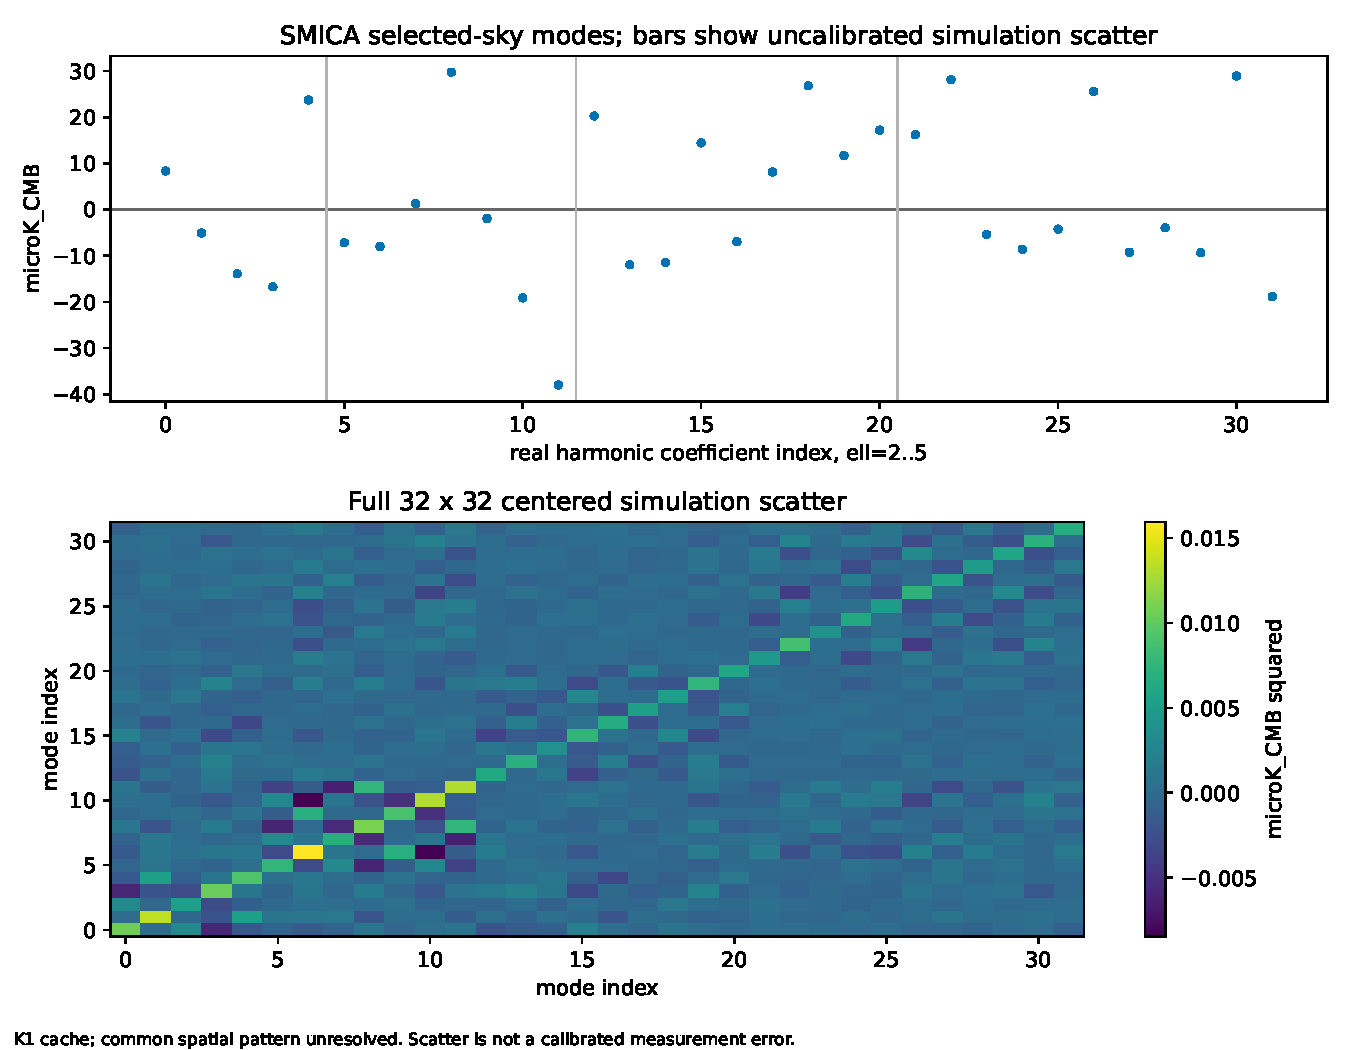
\includegraphics[width=.9\linewidth]{docs/observational_analysis_20261014/results/oa06_smica_scatter_v2/smica_noise_modes.pdf}\caption{Observed low modes and simulation scatter under one K1 processing path. Error bars exclude foreground and shared simulation components.}\end{figure}
\section{Reused descriptive evidence and joint boundary}
The OA02--OA04 CF4 geometry and same-sky CMB contrasts are reused without recomputation. CF4 published group moduli do not supply the selected latent-distance law, velocity covariance, absolute-scale prior or finite-distance remainder required by OA05. OA08's typed DESI summary adapter and OA10's posterior draw interface are tested, but no actual OA09 joint posterior can be formed from the available physical laws. OA11's final physical report remains HOLD.
\begin{figure}[ht]\centering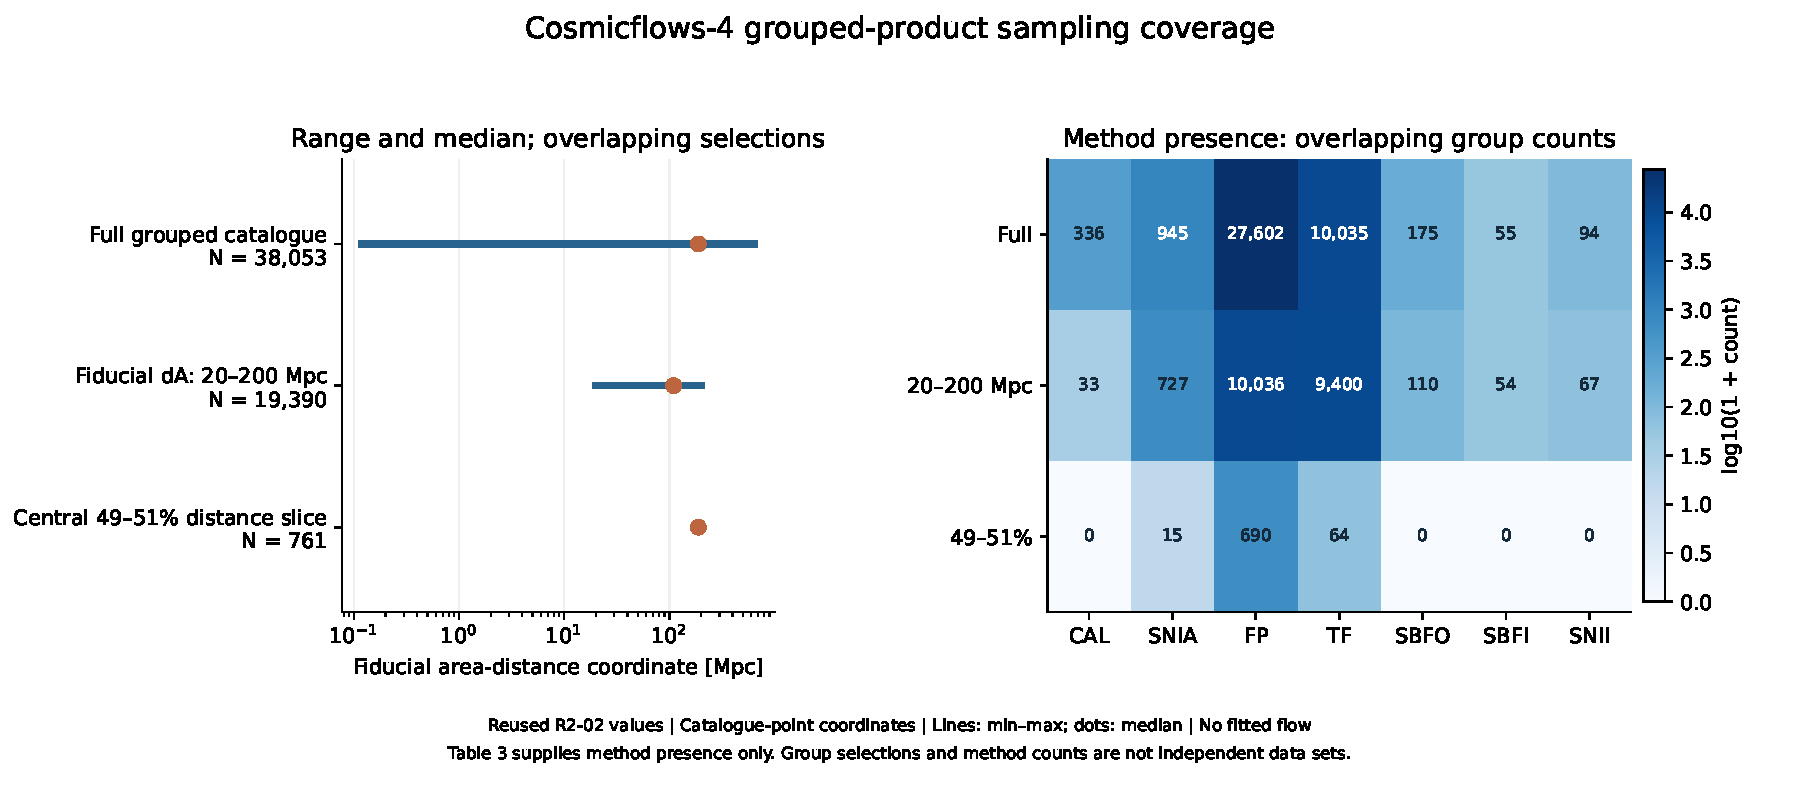
\includegraphics[width=.46\linewidth]{docs/observational_analysis_20261014/results/report/cf4_coverage.pdf}\hfill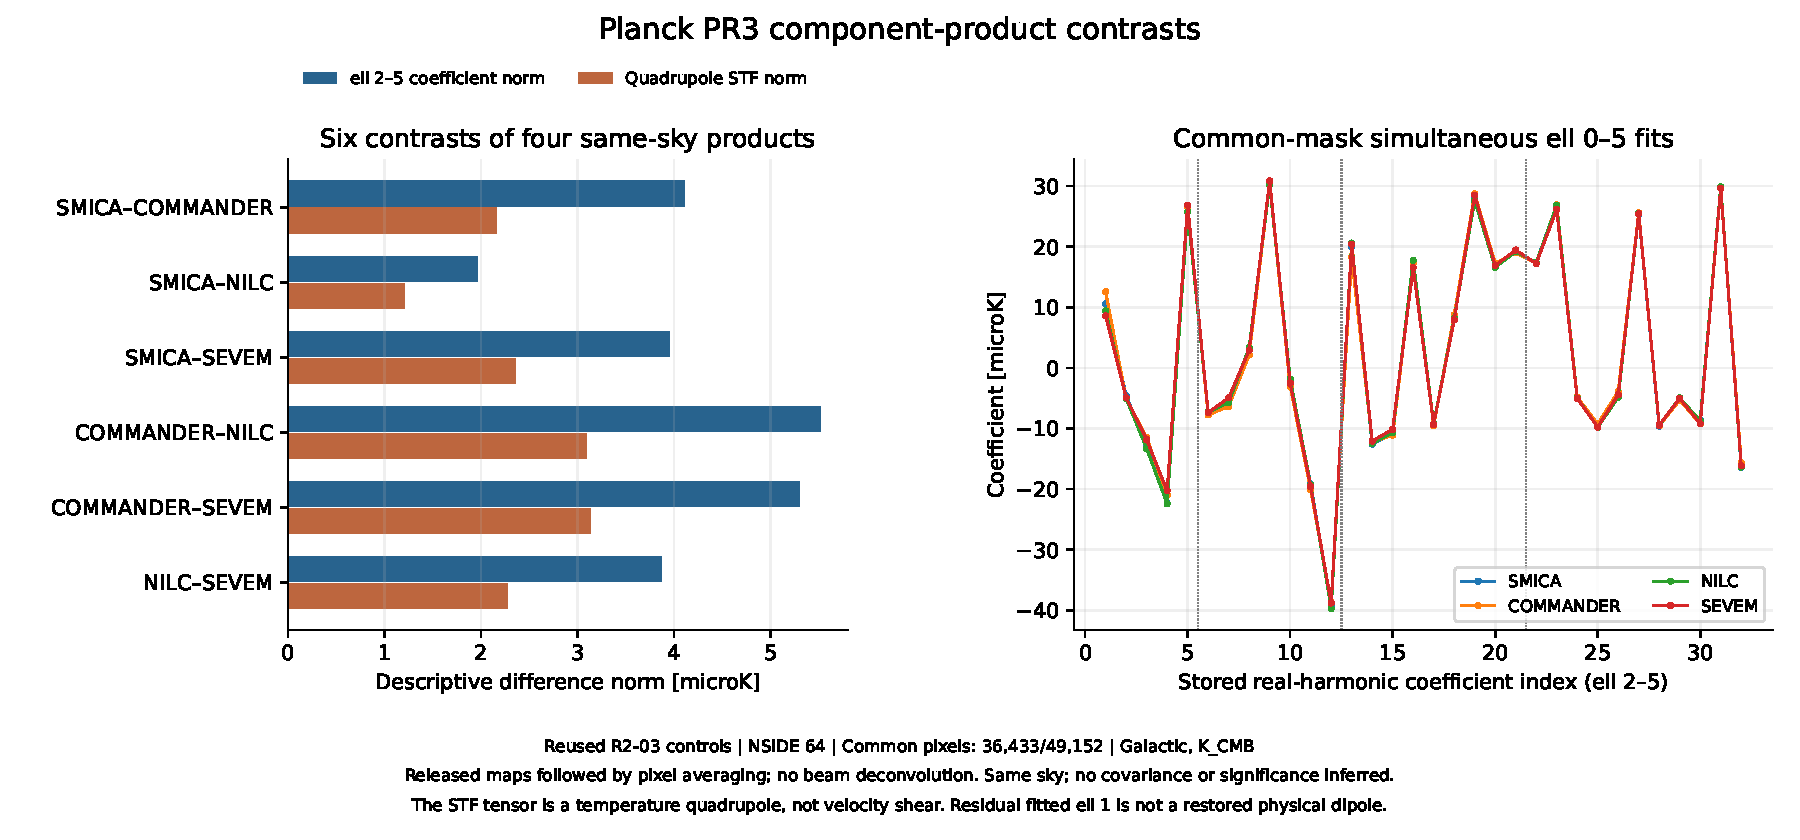
\includegraphics[width=.46\linewidth]{docs/observational_analysis_20261014/results/report/cmb_same_sky.pdf}\caption{Previously accepted descriptive views. Left: CF4 coverage under fixed point-summary geometry. Right: correlated reconstructions of one CMB sky. Neither is a physical joint fit.}\end{figure}
\subsection*{Task status and required physical inputs}
\begin{center}\begin{tabular}{lp{.76\linewidth}}\toprule
Task & Current scope and next input\\\midrule
OA05 & HOLD: selected grouped CF4 law, velocity errors and covariance, shared calibration and scale prior, finite-distance remainder.\\
OA06 & Simulation scatter only: processor response, foreground and systematic covariance, physical low-mode transfer and sky prior.\\
OA07 & Conditional scalar profile; no angular response or separate sound-horizon anchor.\\
OA08 & Typed summary-conditioning adapter tested; actual cross-product dependence and component laws absent.\\
OA09--11 & No joint posterior; posterior pushforward interface and this partial report do not close physical inference.\\\bottomrule
\end{tabular}\end{center}
\paragraph{Provenance.}\mbox{}\par
DESI source digest prefix: \texttt{836a2107c1edfb65}.\par
SMICA cache digest prefix: \texttt{86b792c821b3e641}.\par
Full source digests, numerical values and figure sources are bound in report.json and its named inputs. Scientific admission and native family identification remain HOLD.
\end{document}
